\documentclass{article}

\PassOptionsToPackage{numbers,sort&compress}{natbib}
\usepackage[final]{nips_2016} % produce camera-ready copy
\bibliographystyle{ieeetr}
\usepackage[utf8]{inputenc} % allow utf-8 input
\usepackage[T1]{fontenc}    % use 8-bit T1 fonts
\usepackage{hyperref}       % hyperlinks
\usepackage{url}            % simple URL typesetting
\usepackage{booktabs}       % professional-quality tables
\usepackage{amsfonts}       % blackboard math symbols
\usepackage{nicefrac}       % compact symbols for 1/2, etc.
\usepackage{microtype}      % microtypography
\usepackage{graphicx}
\usepackage{float}
\usepackage{subcaption}
\usepackage{amssymb}
\usepackage{amsmath}
\usepackage{adjustbox}
\usepackage{changepage}
\usepackage{caption}
\usepackage{tabularray}
\UseTblrLibrary{counter,varwidth}
\usepackage{makecell}
\usepackage{enumitem}
\captionsetup{justification=centering}
\usepackage{parskip}


\title{Song Rank Prediction Based on Debut Week Rankings}

% The \author macro works with any number of authors. There are two
% commands used to separate the names and addresses of multiple
% authors: \And and \AND.
%
% Using \And between authors leaves it to LaTeX to determine where to
% break the lines. Using \AND forces a line break at that point. So,
% if LaTeX puts 3 of 4 authors names on the first line, and the last
% on the second line, try using \AND instead of \And before the third
% author name.

\author{
  s2589286\\
  %% examples of more authors
  \And
  s1732775\\
 \And
  s2586913\\
}

\begin{document}

\maketitle


\begin{abstract}
    This study aimed to predict the success of songs on Spotify’s ‘Top 200’ playlist in the near future using a Long Short-Term Memory (LSTM) model, given the song's initial seven-day rankings. Additionally, three other models were trained with additional input features, involving the song's audio features and artists' followers.
    The LSTM model was chosen due to its ability to handle sequential data and its resilience in dealing with skewed datasets, which was a key characteristic of the dataset being used. To evaluate the model performance, the MSE, MAE and $R^2$ scores were computed and compared against two baselines. All models outperformed the two baselines, demonstrating the effectiveness of this approach in forecasting song popularity in the immediate future. Nonetheless, there was no significant improvement in the models trained with the additional input variables compared to the model that used only the seven-day rankings as input.
    
\end{abstract}

\section{Introduction}
According to a 2022 report \cite{spotify_statistics}, Spotify has become the most popular music streaming platform in the world. Its 'Top 200' playlist, also known as charts, consists of the most popular songs streamed on Spotify worldwide. The playlist is updated daily, and the song rankings are based on all-time streams and recent streams \cite{spotifyGeneratePopular}. 
By analysing data about the song's ranking across multiple days on the chart, one can forecast the song's future success or failure in the upcoming days. If the song's rankings are expected to drop, this information may help determine the marketing strategies that could be used to boost the popularity of the song. In addition, such data provides the artist and record label insights about which musical features tend to perform better in terms of remaining high in charts. 

Previously, the forecasting of song success had been done by predicting the daily playback volume for the next 60 days, given historical daily play data of 6 months using long short-term memory (LSTM) models \cite{LSTM_Wang}\cite{LSTM_Random_Forest}. In addition, others have made successful attempts to predict the rank bucket of a song using its audio features and artist popularity measures \cite{sharmaSongPopularity}. In our work, we are interested in predicting the song's success/ranking in the immediate future, given only limited data from the previous seven days. Additionally, our method is inspired by the previously stated studies, where we hypothesise that the song's audio features and the artists' number of followers may be beneficial to the task of forecasting the rankings of the song in the upcoming days.

Thus, we aim to train an LSTM model that predicts the points of a song for the next seven days on the Top 200 playlist, given the points for the initial seven days on the charts, as well as the song's audio features measured internally by Spotify \cite{spotifySpotifyDevelopers}, and artist's popularity, measured as the follower count of the artist.

\section{Data Preparation}
To achieve the intended goal, we utilise a dataset containing the songs from the Spotify ’Top 200’ playlist for each day from 1 January 2017 until 29 May 2023. The dataset contains 651936 rows of songs, each entry containing continuous data of the song’s danceability, energy, loudness, speechiness, acousticness, instrumentalness, and valence, as well as categorical information about the artist/s and their nationalities, song title, song ID and link. The rank in the Top 200 playlist is also included for each song per day, accompanied by the number of points given for such rank (i.e., a song ranked 1st receives 200 points whilst a song ranked 200th receives 1 point), and can be visualised with examples in Appendix \ref{A}.

\subsection{Additional Data Extraction}
We hypothesise that the rankings of a song are highly dependent on the popularity of the artist who released it. Thus, to accurately predict the rankings of a song, we required a measure that illustrates how popular an artist is. Due to the limited data availability in the original dataset, we inspected the documentation of Spotify Web API \cite{spotifySpotifyDevelopers} to obtain additional metrics. It was found that out of the available artist features, the follower count was the most insightful one in terms of describing the artist’s popularity. This was preferred to "Popularity Index" available, as this metric ranges from  0-100 and so would not include the scale of difference in their actual followers, nor provided an indication of how the index was calculated.
To extract such a measure, we first used GET requests to acquire the artist IDs for all unique song IDs in the provided dataset. Further, for each unique artist ID, a GET request was made to obtain the follower count. Lastly, a new column, ‘Followers,’ was added to the original dataset representing the follower count, given the artist in the ‘Artist (Ind.)’ column. The data extraction using the Spotify Web API was performed on the 18th of October. Therefore, the follower counts are accurate as of that date.

\subsection{Abnormality and Missing Value Detection} \label{data_noise}
Upon further inspection of the created dataset, it was observed that the values of the ‘loudness’ feature contained some anomalies. According to the documentation of the Spotify Web API\cite{spotifySpotifyDevelopers}, the loudness should be in the range of -60 and 0 dB. However, most values fell outside this range. By looking at a few sample GET requests to retrieve the loudness of the songs that did not meet the constraint, it was discovered that the values from the dataset that were less than or equal to -1000 were exactly 1000 times less than what the Spotify Web API reported. Thus, the loudness value was divided by 1000 for data points where the loudness was less than or equal to -1000. Four data points where the loudness exceeded 0 were discarded due to inconsistency with the loudness range constraint.

Additionally, it was found that there are four dates within the data collection period when the playlist data is missing. To estimate song’s position on the chart, data imputation was performed by averaging the rank and points from the day before and the day after if the song was present in the respective playlists. Furthermore, there were 104 dates with some rankings missing. To determine which song could potentially be missing, we analysed those songs on the day before and after within a $\pm 50$ rank range that were absent on the given day. By summing up the absolute values of the differences between the song's previous and following day's ranks and the missing rank, we were able to determine the distance to each song. The song with the shortest distance was chosen and placed in the missing rank with its points adjusted. Using this estimation method, seventy missing ranks were filled. The remaining missing ranks are thought as noise in the dataset.

Moreover, some inconsistencies were observed regarding song IDs. Since several songs with identical features and characteristics appear in the chart with multiples songs IDs, song ID cannot be used as a unique song identifying feature. Additionally, for songs that over the course of time exhibit slight alterations in their titles and artist lists, a manual title alignment was performed. 

\subsection{Dataset Restructuring}
The project aims to predict the song’s points over the next seven days, given audio features, the popularity of the song’s artists and points of the seven days since its debut in the chart. Therefore, we performed dataset restructuring such that each dataset point represents a unique song with its respective information. Due to several songs having multiple song IDs, the song title and artist pair measurements were utilised to identify unique songs. 

The new dataset contains 7612 data points with 25 features, including information about the song (title, artists, total followers of artists, chart debut date), audio features (danceability, energy, loudness, speechiness, acousticness,
instrumentalness, valence) and points of the song in charts for 14 days since its debut. More information about each song feature predictor is available in Appendix \ref{D}. If, during any of the 14 days, the song was not apparent in the charts, its point count was set to 0.
Further, we performed Z-score normalisation for all the audio features and total followers. Lastly, the dataset was split into training (90\%) and test (10\%) splits.

\section{Exploratory Data Analysis} \label{EDA}

To gain a deeper understanding of the underlying structure of the newly created dataset, we performed exploratory data analysis (EDA). 
We started by analysing how each of the predictor features relate to target features by evaluating the linear correlation using Pearson’s correlation coefficient.

By observing the correlation matrix in Figure \ref{fig:corr_matrix}, a low to medium positive correlation is noticed between the ‘total follower’ feature and points from day 8 to 14, indicating a potential tendency of songs performed by artists with a higher number of followers achieving higher chart points. Individual audio features and points from day 8 to 14 exhibit a very low correlation, suggesting no linear correlation to determine how well the song will perform during the second week in the charts. The points from day 1 to day 7 and target features have a medium to very strong correlation, demonstrating their viability for being good predictors in determining the points on days 8 to 14. The analysis of the correlation matrix reveals that the points from day 1 to 7 should be considered as main features in the prediction task due to their high correlation with the target features. Although the ‘total follower’ and audio features individually exhibit a low correlation with the target variables, it is plausible that the combination of them together with points features might yield sensible results.

\begin{figure}
    \centering
    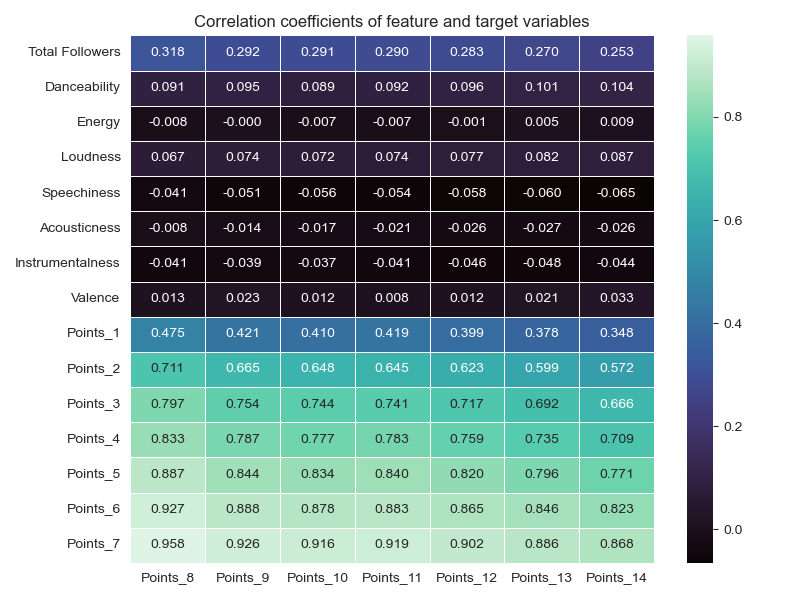
\includegraphics[width=0.7\textwidth]{figures/correlation_matrix.png}
    \caption{Correlation matrix of feature and target variables. The vertical axis illustrates feature variables, whereas the horizontal axis illustrates target variables.}
    \label{fig:corr_matrix}
    
\end{figure}

We begin the examination of distribution of the predictor variables by analysing the histograms ‘total followers’ and the audio features in Figure \ref{fig:fol_aud_hist}.  The distributions of ‘total followers’, ‘speechiness’, ‘acousticness’ and ‘instrumentalness’ all are strongly right-skewed, whereas ‘danceability’, ‘energy’ and ‘loudness’ are moderately left-skewed. ‘Valence’ is the only feature with a distribution similar to normal.  Due to the high number of predictor points features, we illustrate only three of them (Figure \ref{fig:pred_p_hist}), with the remaining ones exhibiting behaviour akin to that of days two and seven. The distribution of points on day one is rightly skewed, suggesting that song enter the chart at a low position. Similarly, day two and day seven point distributions have a right skew with a major peak at value 0, indicating that many songs leave the chart soon after entering it.
Figure \ref{fig:targ_p_hist} illustrates the distribution of three target points features, which are similar in distribution to the points on days two and seven


\begin{figure}
  \begin{adjustwidth}{-2cm}{-2cm}  % Adjust these values as needed
    \centering
    \begin{minipage}[b]{0.5\linewidth}
      \centering
      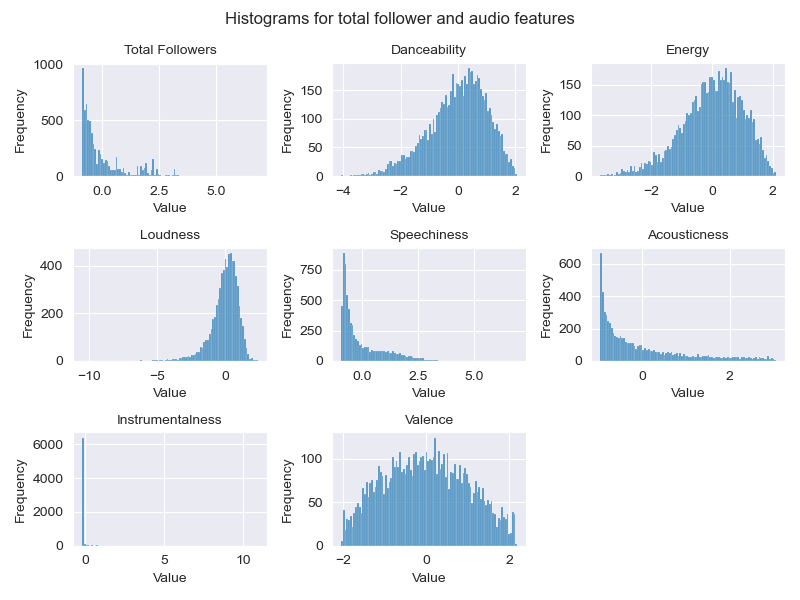
\includegraphics[width=\linewidth]{figures/fol_audio_hist.png}
      \caption{Frequency distribution histograms of total followers and audio features.}
      \label{fig:fol_aud_hist}
    \end{minipage}%
    \begin{minipage}[b]{0.5\linewidth}
      \centering
      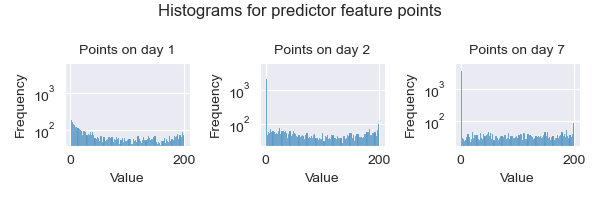
\includegraphics[width=\linewidth]{figures/predict_point_hist.png}
      \caption{Log-scale frequency distribution histograms of points on days 1,2 and 7.}
      \label{fig:pred_p_hist}

      \vspace{4mm} % Adjust the space between the images

      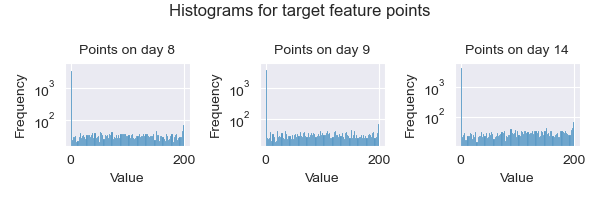
\includegraphics[width=\linewidth]{figures/target_point_hist.png}
      \caption{Log-scale frequency distribution histograms of points on days 8,9 and 14.}
      \label{fig:targ_p_hist}
    \end{minipage}
  \end{adjustwidth}
\end{figure}


\section{Learning Methods}
\subsection{Model Selection}
To tackle the task of predicting the points of a song for the second week, we opt to use an LSTM model \cite{original_LSTM}, a type of recurrent neural network (RNN). Its architecture is designed to effectively capture long-term dependencies, making it well-suited for time series analysis. This characteristic is crucial for our task, as we aim to predict the song's points over the next seven days, where understanding the temporal dynamics in the first seven days since the song's debut on the chart is essential \cite{LSTM_paper}. Additionally, our choice of the LSTM model is rooted in the key consideration that the nature of our data is characterised by significant skewness. Thus making it necessary to use a robust neural network approach. LSTM is a subtype of the neural networks model family, which theoretically can approximate any function\cite{NNcancomputeanyfunction}, alleviating the issue of a skewed dataset.
Lastly, LSTM models have shown success in similar song rank prediction tasks \cite{LSTM_Wang}\cite{LSTM_Random_Forest}. Thus, we consider it an appropriate choice for the set task.

\subsection{Model Types and Architecture}
Our research aims to determine whether it is possible to forecast the song's chart points for the second week based on the first week's points and whether adding the song's audio and follower attributes improves the model's performance. Thus, we require the training of four distinct models, each using different combinations of input features:

\begin{itemize}[leftmargin=10pt]
  \item[] \textbf{Model 1}: song's points for the first 7 days since its debut in the chart. 
  \item[] \textbf{Model 2}: song's points for the first 7 days since its debut in the chart and audio features.
  \item[] \textbf{Model 3}: song's points for the first 7 days since its debut in the chart and artists' followers.
  \item[] \textbf{Model 4}: song's points for the first 7 days since its debut in the chart, audio features and artists' followers.
\end{itemize}

To develop the intended LSTM models, we utilise the TensorFlow and Keras libraries. We build a single-shot LSTM architecture, where the whole target sequence is predicted during the last time step \cite{tensorflowTimeSeries}. The architecture consists of a single LSTM unit whose output is fed into a fully connected layer. 

The model input features are pre-processed such that every data sample represents a single song with seven time steps representing the first week on the chart. For Model 1, each time step represents the points on the respective day. Whereas for Models 2,3 and 4, the time steps are vectors containing points on the day along with audio features and/or follower count. The model targets for every data sample are the song's chart points during the second week.
 
\subsection{Hyperparameter Search and Training}

In order to find the hyperparameter set that results in the best-performing model for every Model type, we conduct a grid search with possible $batch\_size \in \{32,64,128,256\}$, $epochs \in \{10n | 1 \leq n \leq 15, n \in \mathbb{Z}\}$ and $hidden\_units \in \{32,64,128,256,512\}$ values. The rest of the hyperparameters for the LSTM unit and fully connected layer remain default as in the Tensorflow and Keras libraries\cite{TF_LSTM}\cite{TF_Dense}.

To enhance the reliability of our model evaluation, the hyperparameter search was conducted using $k$-fold cross-validation with $k = 10$. The training dataset was split into ten subsets, with each iteration using nine subsets for training and one for validation. This process was repeated ten times to ensure that each subset serves as both training and validation data. During each iteration, the dataset was normalised using Z-score normalisation, maintaining consistency in feature scaling across folds. For each set of hyperparameters, after completing all folds, we aggregate the training histories to derive average loss (MSE) and MAE metrics. 

The first step in determining the optimal set of hyperparameters is finding the epoch that yields the best model generalisation (smallest training and validation loss) for each batch size, hidden units pair. Out of those selected, the hyperparameter set resulting in the lowest MAE was chosen. In order to reduce the number of hidden units used in our model, if the lowest MAE was associated with 256 or 512
hidden units, then a different combination of hyperparameters was chosen if their MAE fell within
$\pm2.5 \% $ range of the lowest MAE. 

The found hyperparameter combination is then used to train the model on the full training set. 


\section{Results and Evaluation}
This section describes the evaluation metrics and comparative baselines used to assess the 4 LSTM model performance.

\subsection{Evaluation Metrics}
In regression analysis, various evaluation metrics are employed to assess the performance of predictive models, including (1) Mean Squared Error (MSE), (2) Mean Absolute Error (MAE), and (3) R-squared ($R{^2}$).
MSE and MAE are valuable for understanding the magnitude and distribution of errors, while $R{^2}$ provides insights into the overall model fit.

\subsection{Baseline Models}

To gauge the effectiveness of our LSTM models, their performance is compared against two baseline models, which consist of:

\begin{itemize}[leftmargin=10pt]
  \item[] \textbf{Baseline 1}: Predicts the same points of day 7 for the next 7 days. Since many songs have 0 points on days 7–14, this model was adopted in order to provide reliable estimates.

  \item[] \textbf{Baseline 2}: Predicts the points for the next 7 days using a linear function fit between day 1 and 7 points. Since the predictor and target feature variables have a medium-to-strong linear correlation (Section \ref{EDA}), we expect to see accurate forecasts.

\end{itemize}

\subsection{Optimised Hyperparameters}
After conducting the hyperparameter search, we find that the best (hidden unit, batch size, epoch) hyperparameter sets for LSTM Models 1-4 are: (32, 32, 130), (128, 32, 40), (32, 32, 150), and (256, 64, 50) respectively. The details of the best hyperparameter selection process are available in the Appendix \ref{B}, with additional insights into the best hyperparameter sets available in Appendix \ref{C}.




\subsection{Model Evaluation}
Evaluation was carried out by testing each LSTM model and baseline model on the test dataset. Using the optimsed hyperparameters, MSE, MAE and $R{^2}$ were used to compare the LSTM models to baseline models. As seen in the summary Table \ref{tab:test}, all four LSTM models outperformed both baseline models, suggesting that the LSTM architecture is learning based on charts of the first 7 days of the input song and is suitable for predicting the next 7 chart days. However, inclusion of the audio features and artist followers did not seem to improve the model.

\begin{table}[h!]
  \centering
  \begin{tabular}{|p{6cm}|c|c|c|}
    \hline
    \textbf{Model} & \textbf{Test dataset MSE} & \textbf{Test dataset MAE} & \textbf{$R{^2}$}\\
    \hline
    Baseline 1 & 750.84 & 13.15 & 0.81 \\
    Baseline 2 & 675.24 & 11.81 & 0.83 \\
    Model 1: points only & 371.19 & 9.62 & 0.91 \\
    Model 2: points, audio features & 391.74 & 9.90 & 0.90 \\
    Model 3: points, followers & 364.05 & 9.73 & 0.91 \\
    Model 4: points, audio features, followers & 387.51 & 10.00 & 0.90 \\
    \hline
  \end{tabular}
  \caption{Summary of MSE, MAE, and $R{^2}$ of test dataset on each 4 models, taking optimised hyperparameters for each model. Baseline models are also included.}
  \label{tab:test}
\end{table}

The MAE of the test dataset were compared between each model to the best performing baseline model (linear function baseline model) by using one-tailed t-tests. All four models' MAE were significantly lower than the best performing baseline model MAE, i.e. the linear function baseline model. This indicates that the null hypothesis that the LSTM models perform equally as well as Baseline model 2 can be rejected. Summary data of these statistical tests can be found in Appendix \ref{D}.


\subsection{Discussion}
LSTM has shown to be efficient for modelling time-series Spotify song data to predict popularity over the next 7 days, given the popularity of the initial 7 days on the charts. 

Despite EDA indicating that artist total followers may also influence song points on Spotify charts, including artist followers in combination with first 7 day points as well as in addition to audio features (models 2 \& 4) did not appear to improve performance of the test dataset on the LSTM model. However, this may be impacted by the abnormalities detected in the dataset as mentioned in Section \ref{data_noise}. Moreover, acquisition of artist follow counts was carried out in one batch on 18th October. This implies that this predictor did not capture the true number of followers of the artist on the day of each song release in the dataset. The inconsistency within the dataset led to irregularities in the "Artists" column, occasionally resulting in the omission of collaborative artists and featuring only a single artist for songs involving collaboration. Moreover, including song audio features appears to also not sufficiently improve the model, indicating that the progression of popularity of a song is mainly dependent on its popularity trend on the first 7 days of charting, with audio features have low weight in the model. This may be due to the method of how the song features were encoded into the model, in which they were added for every time step instead of once per song. Also, the training data spanned over 6 years, where the prevalent audio features in songs has likely not drastically changed. This could be improved and contrasted to song popularity data over tens of years, where genre popularity has substantially changed, implying song audio features also have. In this case, they may have a more crucial role in training the LSTM model and determining song popularity.

Additionally, limitations with the data that hinder model training include the presence of songs that were released before the establishment of Spotify and subsequently added to Spotify during the years included in data collection (2017-2023), and songs that were released on Spotify before 2017 but still charted during the data collection period. Besides an artist's pre-existing popularity, trends that rapidly gain popularity on social media platforms such as TikTok also have significant impact on the popularity of a song, generally regardless of song audio feature of artist popularity \cite{TikTok}. Furthermore, even though an LSTM model is optimal for modelling skewed daily points data, this skewness nonetheless affects the performance of the model. 


\section{Conclusion}

This paper involves training an LSTM model to predict the popularity of Spotify songs for the following 7 days, based on the initial 7 days on charts. This input of time-series data involves highly skewed  points per day, so is suited to be modelled by LSTM. We evaluated 4 LSTM models, involving predictors of (1) points only, (2) points and audio features, (3) points and artist followers, and (4) points, audio features, and artist followers. These models were evaluated by comparing MSE, MAE, and $R{^2}$ to baseline models, in which all models achieved a significantly lower MAE in comparison to the best-performing baseline model. However, neither audio features or artist followers appeared to improve the model when added as predictors. This model could be improved further by testing alternative model architectures and different predictor feature encoding types. 
 Furthermore, including data over a longer number of years may be beneficial in inferring change in popularity of audio features over time, related to change in genre popularity.
\newpage
\bibliography{refs.bib}
\bibliographystyle{plain}
\newpage
\section*{Supplementary Information}
\subsection{Contribution list}
\begin{enumerate}
    \item \textbf{s2589286}
 \newline For the paper, I contributed to:
  \begin{itemize}
      \item Writing 'Data Preparation' and 'Exploratory Data Analysis' sections.
      \item Providing a list of necessary information for the 'Learning Methods' section and its refinement.
      \item Proofreading and minor adjustments of the whole report.
    \end{itemize}
  For the project development, I:
  \begin{itemize}
  \item Performed additional data collection using Spotify API.
  \item Performed dataset cleaning and restructuring, including EDA.
  \item Implemented the model using Tensorflow and Keras libraries.
  \item Contributed with ideas and suggestions for model development and improvement.
  \end{itemize}
  
    
    \item \textbf{s1732775}
  \newline For the paper, I contributed to:
  \begin{itemize}
      \item Writing and gathering references for the abstract and learning methods, and appendices E and F sections;
      \item Proofreading the introduction section.
  \end{itemize}
In terms of the project, I contributed to:
  \begin{itemize}
      \item Researching the algorithms and machine learning techniques to use and the details for implementation, as well as gathering and sharing learning resources with my teammates;
      \item Learning to use Eddie, the University of Edinburgh's super computer, and used it to fine-tune LSTM hyperparameters;
      \item Booking rooms for weekly meetings.
  \end{itemize}
  
    \item\textbf{s2586913}
    \newline For the paper, I contributed to:
  \begin{itemize}
  \item Writing of Introduction, Evaluation Metrics, Discussion, Conclusion, and Appendices, as well as generating figures and tables.
  \item Proofreading the whole report with additions of small components throughout.
  \end{itemize}
In terms of the project, I:
  \begin{itemize}
  \item Contributed and implemented ideas and suggestions for the direction of the project and aim
  \item Reviewed the literature to determine commonly used machine learning methods for time-series data
  \item Aided with optimising hyperparameters for each model
  \item Carried out statistical testing of the MAE evaluation metrics

  \end{itemize}
\end{enumerate}


\subsection{Generative AI}

We made use of generative AI to generate ideas of how to include the additional predictors of audio features and artist followers in an LSTM model, when dealing with time-series data of points per day.

\newpage
\section*{Appendices}

\appendix
\section{Training Set at a Glance}\label{A}

To illustrate the time series nature of the points' features, we provide the points for the first 14 days since the song's debut in the chart of 10 randomly sampled songs shown below.  

\begin{figure}[H]
    \begin{adjustwidth}{-2cm}{-2cm}
    \centering
    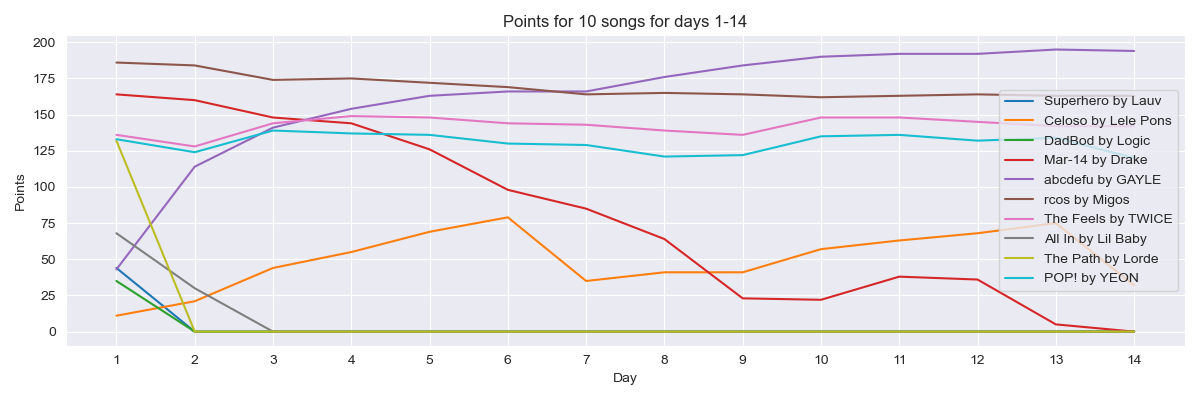
\includegraphics[width=1\linewidth]{figures/10_song_points.png}
    \caption*{Points for the first 14 days since the song's debut in the chart of 10 randomly sampled songs.}
    \label{fig:10_songs}
    \end{adjustwidth}
\end{figure}

\section{Available Hyperparameters}\label{B}

All the combinations of number of hidden units and batch size are paired with the corresponding epoch number associated with the smallest loss in the test set. These were picked by identifying instances where the loss remained constant for two consecutive epochs, in which the second epoch was chosen. This was done to prevent over-fitting of the model, and can be seen in the figure above. The table below is an example of all the combination of these hyperparameters, with the corresponding MAE, by using that of LSTM model 1 with only points used as a predictor. In this case, 32 hidden units, a batch size of 32, and 130 epochs were chosen as the optimised hyperparameters for model 1, as they are assocaited with the lowest MAE.

\newpage
\begin{figure}[H]
    \begin{adjustwidth}{-1.5cm}{-1.5cm}
    \setkeys{Gin}{width=\linewidth}
    \begin{tblr}{colsep=4pt,
             colspec={@{} *{4}{X[c]}@{}}, 
             measure = vbox}
     
            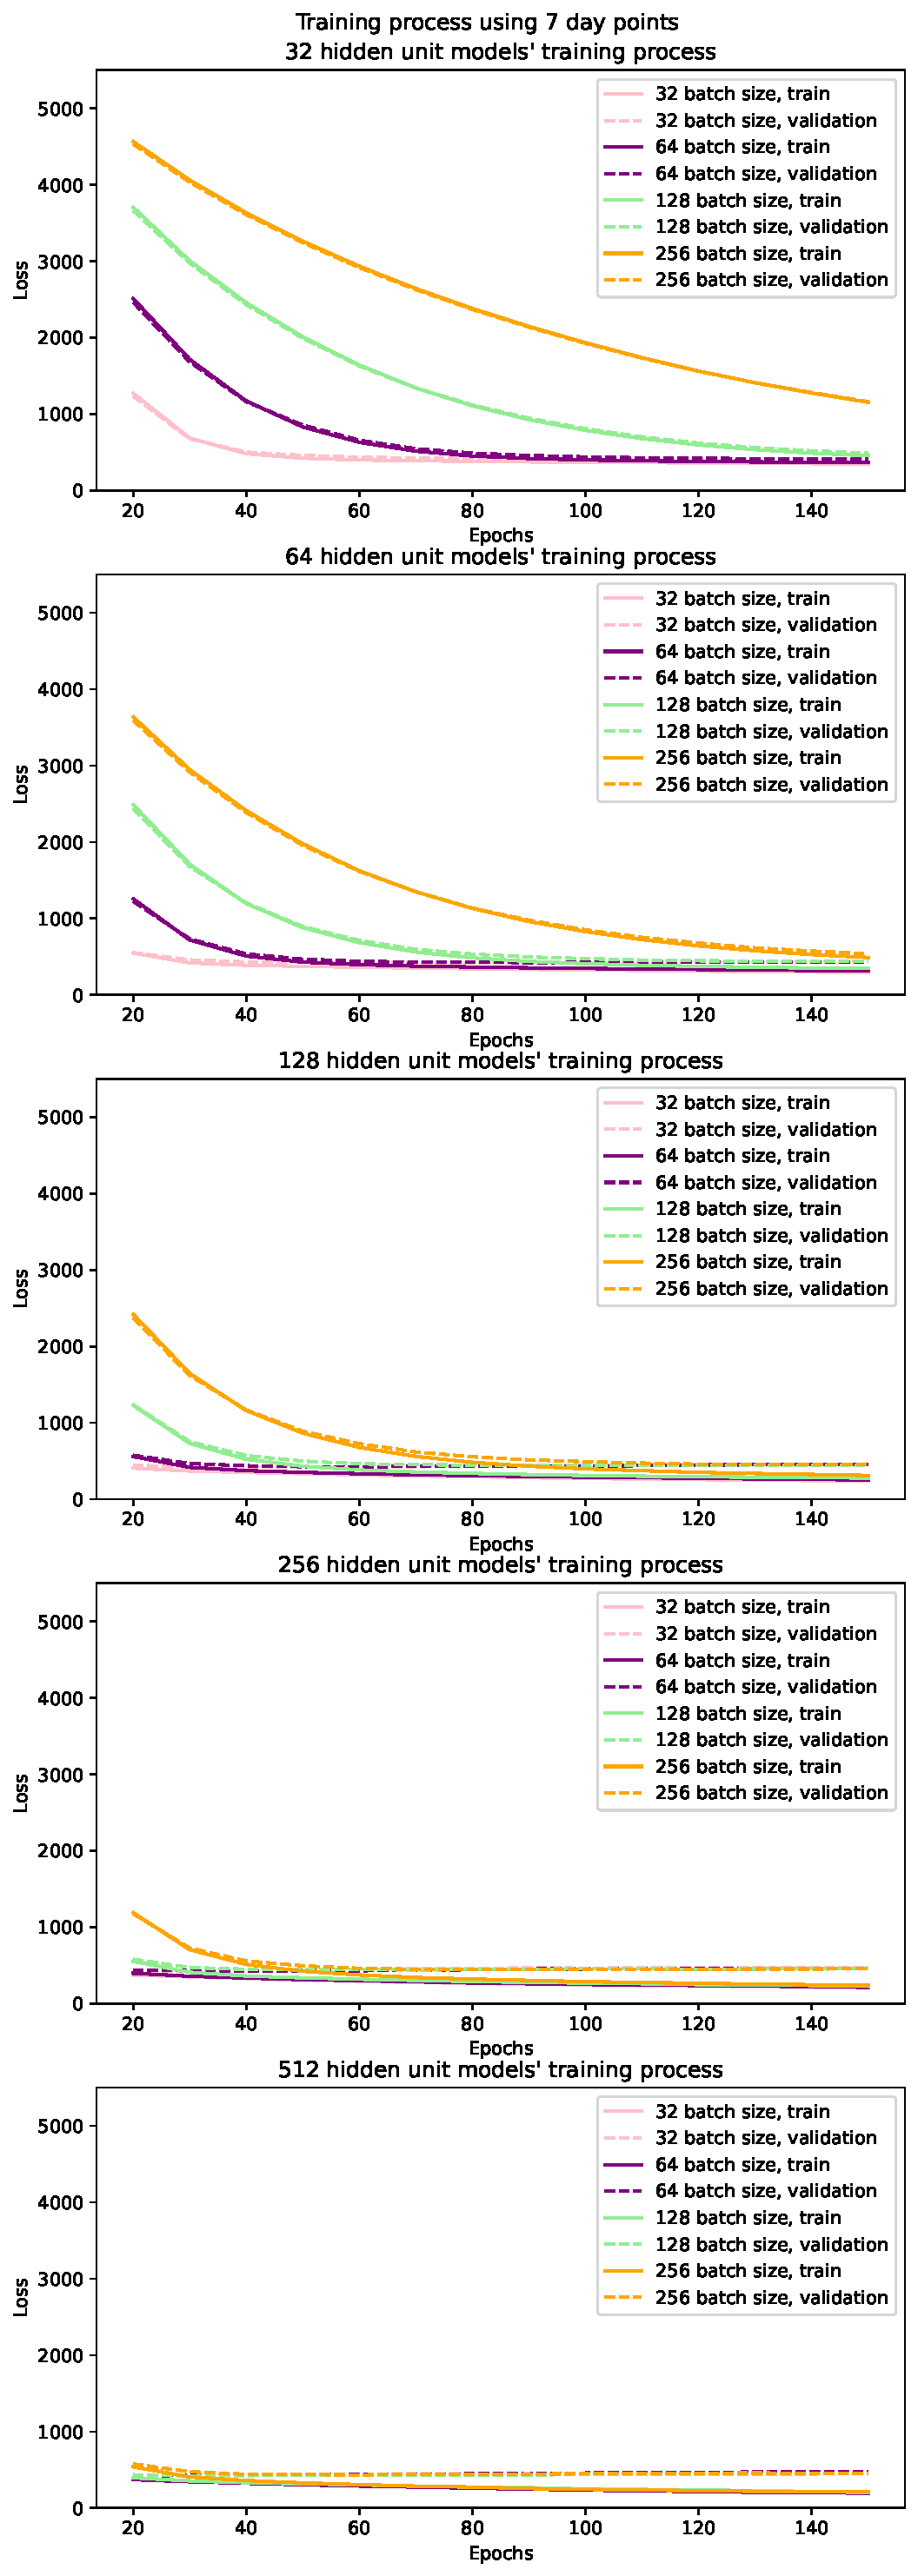
\includegraphics[width=\linewidth]{figures/hyperparameters_points_training.pdf}
            \caption{LSTM model taking first 7 day points as the only predictors.}
            \label{fig:hyper1}
        
        &
        
            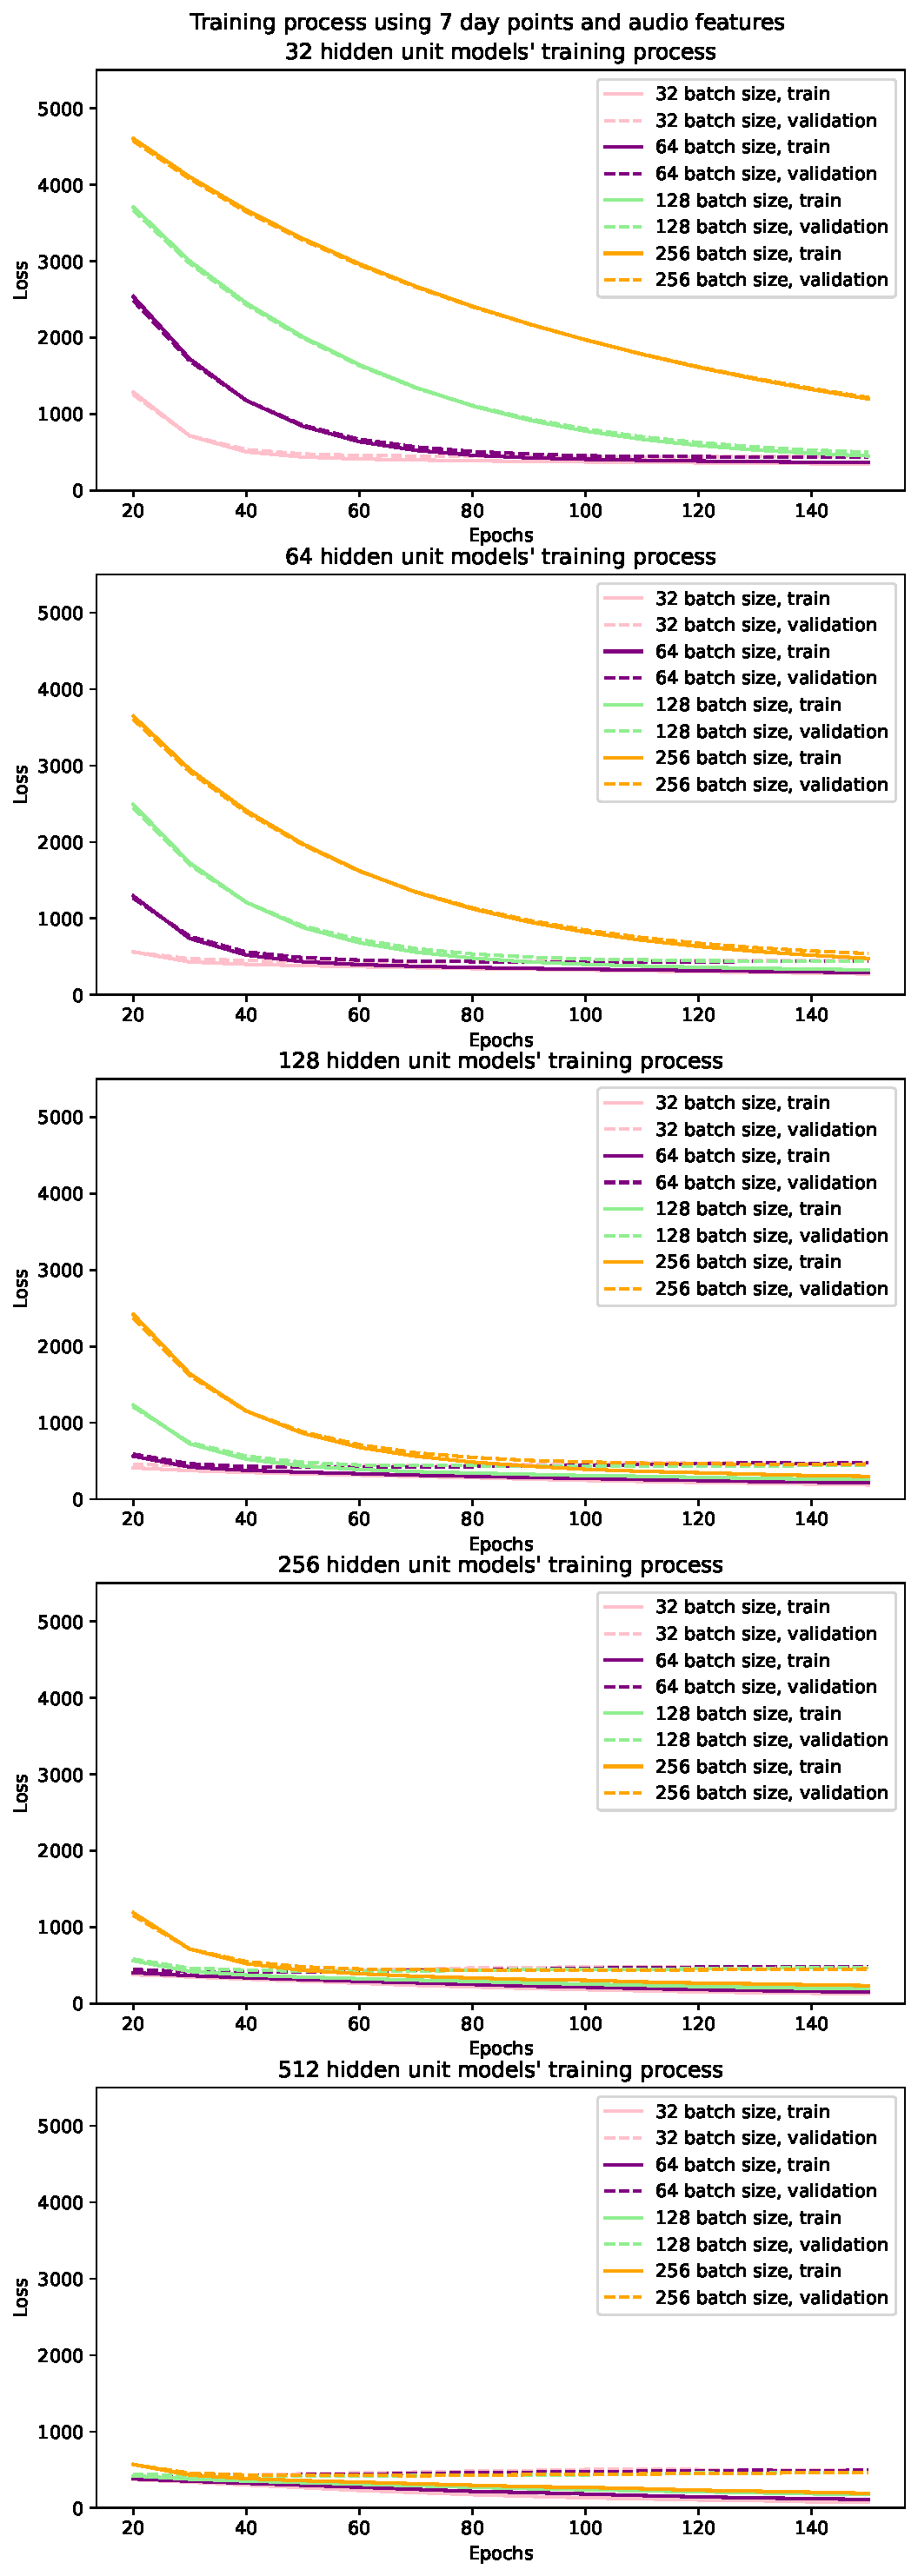
\includegraphics[width=\linewidth]{figures/hyperparameters_points_audio_training.pdf}
            \caption{LSTM model taking first 7 day points and audio features as predictors.}
            \label{fig:hyper2}
        
        &
        
            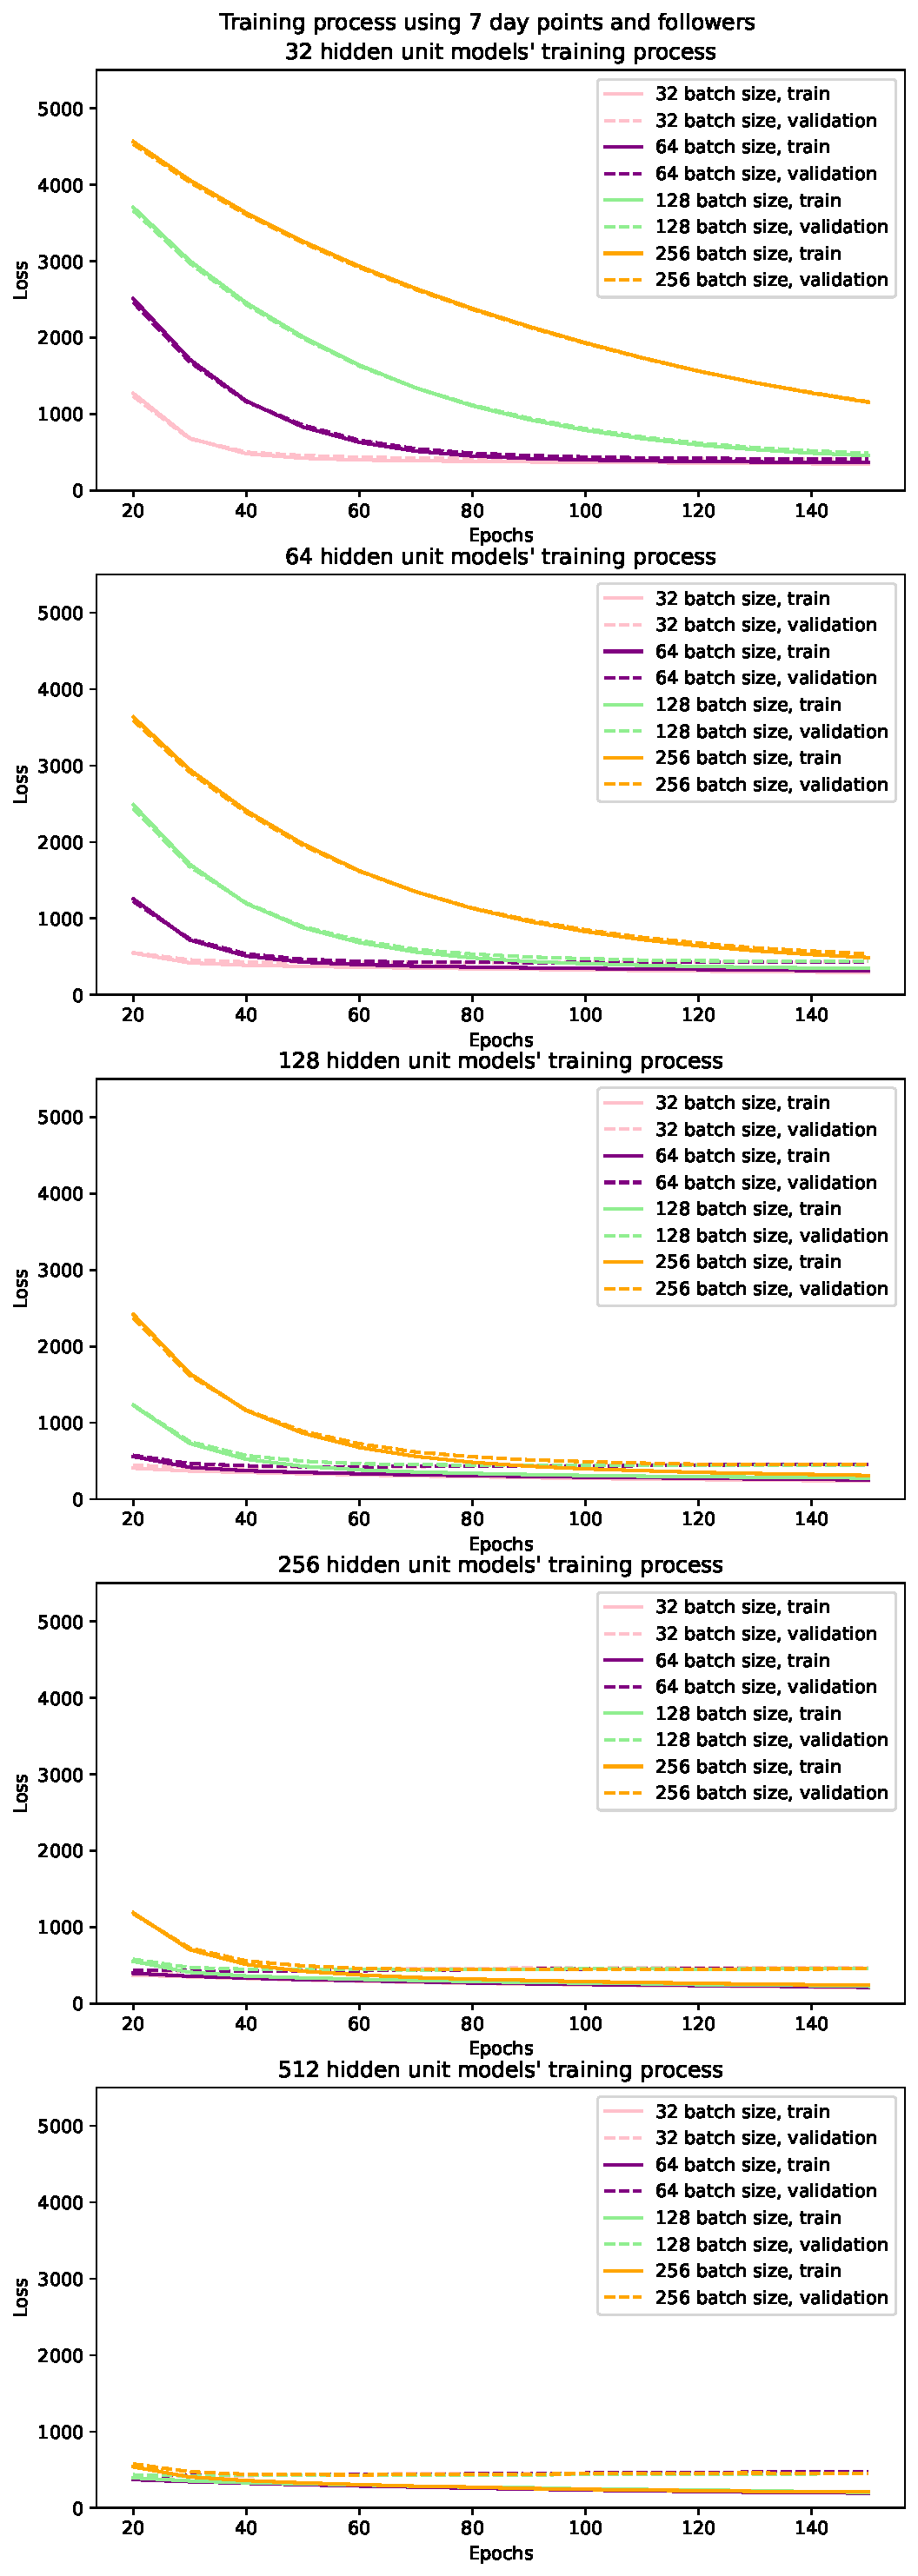
\includegraphics[width=\linewidth]{figures/hyperparameters_points_followers_training.pdf}
            \caption{LSTM model taking first 7 day points and followers as predictors.}
            \label{fig:hyper3}
        
        &
       
            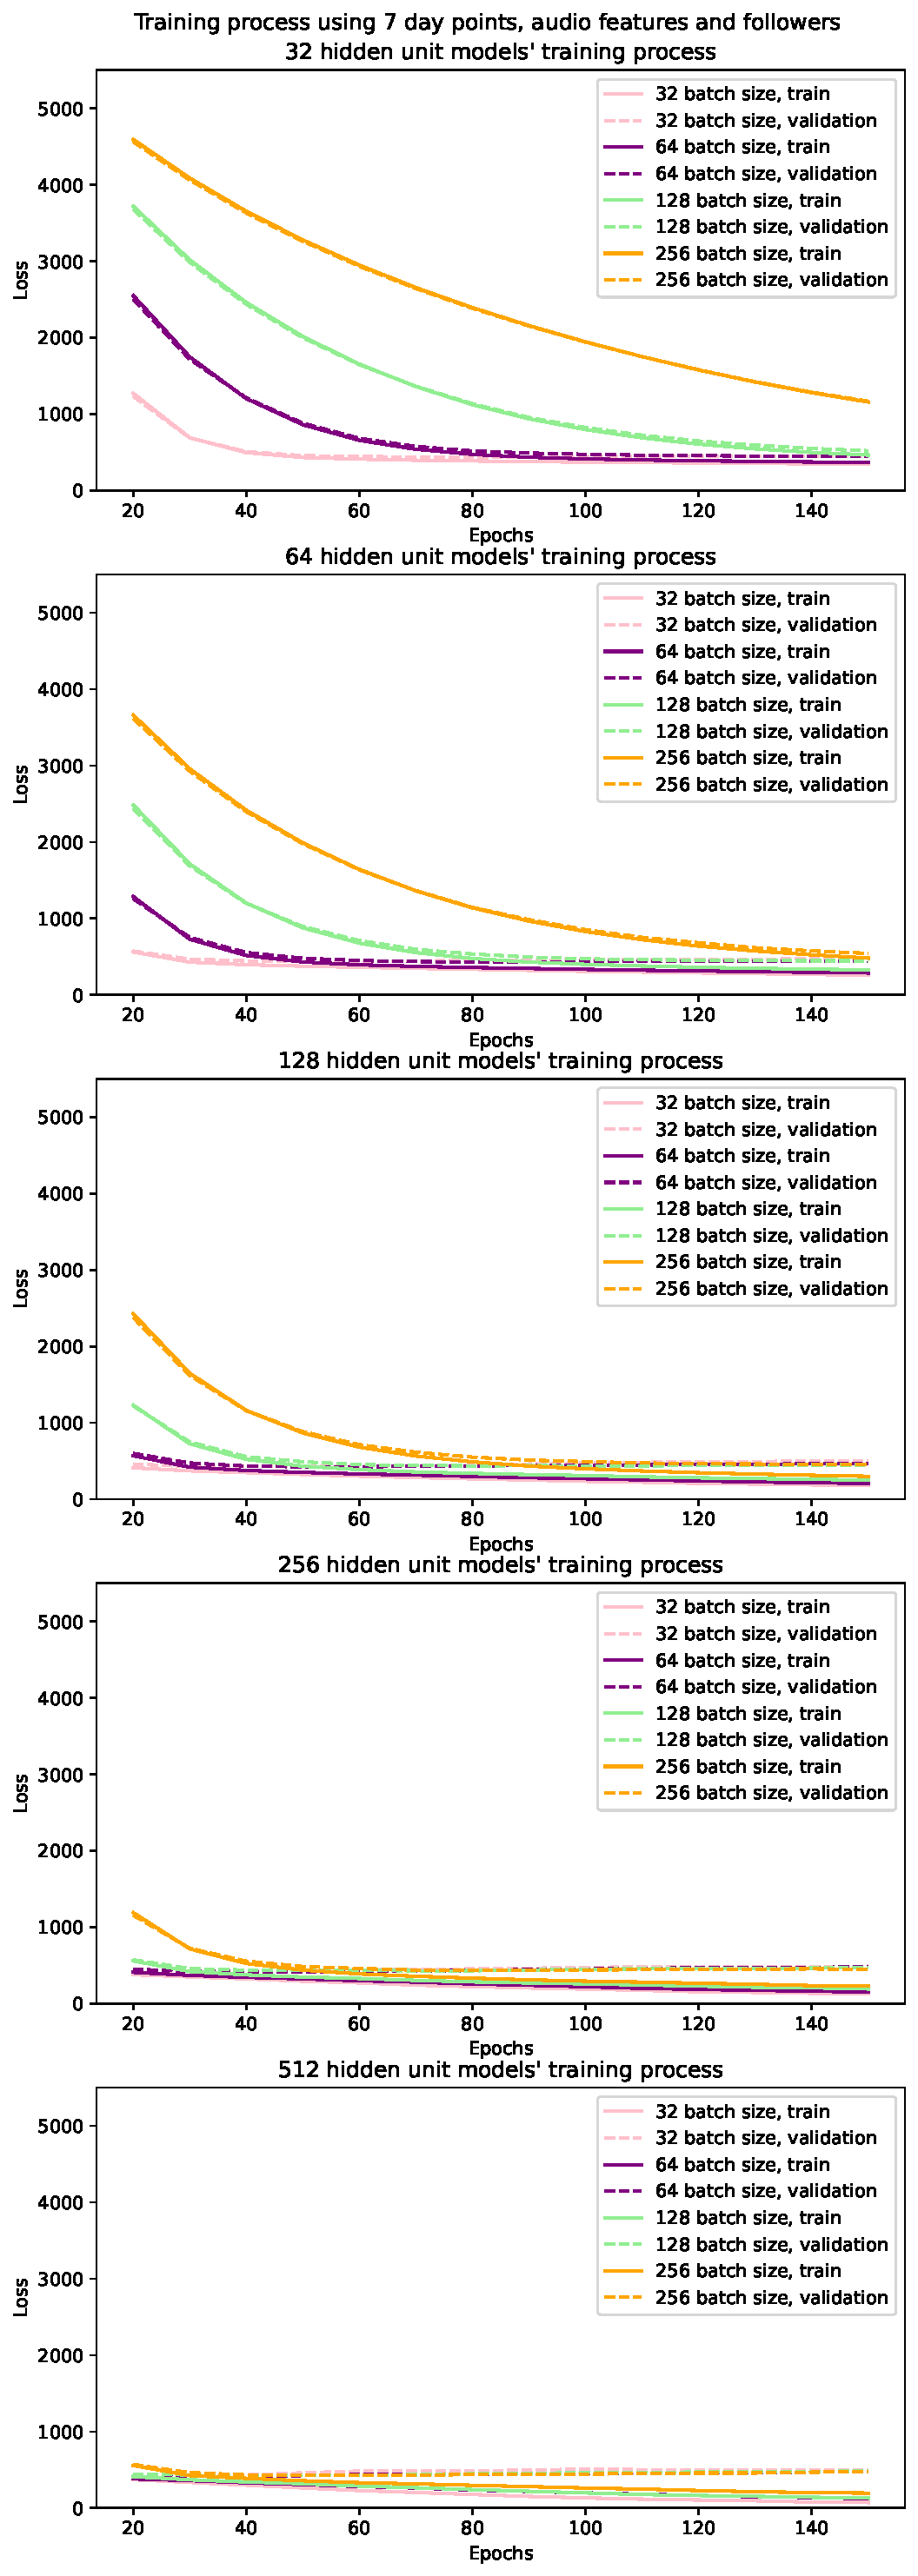
\includegraphics[width=\linewidth]{figures/hyperparameters_points_audio_followers_training.pdf}
            \caption{LSTM model taking first 7 day points, audio features, and followers as predictors.}
            \label{fig:hyper4}
      
\end{tblr}
        \caption*{Test set loss vs epoch number for various combinations of hidden units and batch size for all 4 LSTM models.}
        \label{fig:hyper}
    \end{adjustwidth}
\end{figure}


\begin{table}[H]
  \centering
  \begin{tabular}{|c|c|c|c|}
    \hline
    \textbf{Hidden Units} & \textbf{Batch Size} & \textbf{Epoch number} & \textbf{Test Set MAE}\\
    \hline
    32&32&130&10.581\\
    32&64&150&10.72\\
    32&128&	150&12.739\\
    32&	256&150&20.385\\
    \hline
    64&32&80&10.722\\
    64&	64&90&10.851\\
    64&128&150&11.178\\
    64&256&150&13.408\\
    \hline
    128	&32&40&10.755\\
    128	&64&60&	10.864\\
    128&128&130&10.915\\
    128	&256&140&11.521\\
    \hline
    256&32&20&10.836\\
    256&64&40&10.813\\
    256&128&70&11.057\\
    256&256&110&11.127\\
    \hline
    512&32&20&10.803\\
    512&64&20&10.813\\
    512&128&30&10.962\\
    512&256&60&11.159\\
    \hline
  \end{tabular}
  \caption*{Hyperparameter combinations of hidden unit number, batch size and epoch numbers with corresponding test dataset MAE for LSTM model 1, that includes only the first 7 days of points as predictors.}
  \label{tab:hyper_combos}
\end{table}

\section{Fine-tuned Hyperparameters}\label{C}

\begin{table}[H]
  \centering
  \begin{tabular}{|p{5cm}|c|c|c|c|}
    \hline
    \textbf{LSTM Model} & \textbf{Hidden Units} & \textbf{Batch Size} & \textbf{Epochs} & \textbf{\makecell{Training \\ set MAE}}\\
    \hline
    (1) Points only & 32 & 32 & 130 & 10.58 \\
    (2) Points, audio features & 128 & 32 & 40 & 10.72 \\
    (3) Points, followers & 32 & 32 & 150 & 10.61 \\
    (4) Points, audio features, followers & 256 & 64 & 50 & 10.55 \\
    \hline
  \end{tabular}
  \caption*{Summary of best set of hyperparameters per model, involving the average lowest MAE on training datasets using a K-fold of 10, with corresponding number of hidden units, batch size, and associated epoch number.}
  \label{tab:hyper}
\end{table}



\section{Statistical testing of the Evaluation metric}\label{D}

\begin{table}[H]
  \centering
  \begin{tabular}{|c|c|c|}
    \hline
      &  \multicolumn{2}{|c|}{\textbf{vs Linear Function Baseline Model}}\\ \hline 
    \cline{2-3}
    \textbf{LSTM Model} & \textbf{t-Statistic} & \textbf{\textit{p}-Value} \\
    \hline
    (1) Points only & -11.97 & 6.67E-33*** \\ 
    (2) Points, audio features & -38.44 & 6.41E-286*** \\ 
    (3) Points, followers & -36.69 & 2.67E-263*** \\ 
    (4) Points, audio features, followers & -37.95 & 1.57E-279*** \\ \hline
    
  \end{tabular}
  \caption*{Statistical testing using one-tailed t-tests of test dataset LSTM model MAE compared to the linear function baseline model MAE. Summarised are the t-statistics and p-values. ***\textit{p} < 0.001 }
  \label{tab:ttest}
\end{table}

\section{Additional Ideas for Completion}\label{E}

These are the further ideas that we didn't implement due to the lack of time:
\begin{enumerate}
    \item \textbf{Classification for determining impactful features}
\newline There are seven audio features for each song in the dataset, and not all of them are equally important when it comes to predicting the future rankings of a song. Hence, it is important to select which features are likely to impact the popularity of a song. For this purpose, we can use a few classification algorithms: Decision Tree, Random Forest and k-Nearest Neighbour. After deciding on the best classification algorithm to use, we can then use a grid search method to fine-tune them before proceeding to training the neural network. The grid search function from scikit-learn library \cite{scikit-learn} performs an exhaustive search over a specified hyperparameter grid to find the best combination of hyperparameters for a machine learning model. The function systematically trains and evaluates the model with possible hyperparameters using K-fold cross-validation, where the dataset is split into ‘k’ subsets, and the model is trained and evaluated ‘k’ times. Finally, it returns the best set of hyperparameters that yield the highest cross-validated performance, which then allows fine-tuning of the classifier. After this step, we will be able to identify the most likely features to predict a song’s rankings and the least likely ones. The most impactful features will then be used as the training data in the LSTM model training step to predict a song’s ranking trend based on its features. For evaluating the classifiers used, we will employ ROC-AUC \cite{ROC-AUC}.
After screening for the most impactful audio features, we can build models with individual audio features instead of using a mix of all of them, to see whether any individual audio feature stands out to be prevalent to predict song popularity. 
    \item \textbf{Use of an Autoregressive Integrated Moving Average (ARIMA) model for time series}
\newline For future work, we could consider implementing an ARIMA model \cite{ARIMA} to forecast the rankings of songs on the Spotify ‘Top 200’ playlist. The ARIMA model could be particularly useful in our context of predicting song popularity. Given that song popularity is a time series data, the ARIMA model can capture the temporal dependencies and trends in the data, making it a strong candidate for further exploration.

This would involve training the model on the historical ranking data, and using it to predict future rankings. The model’s predictions could then be compared with the actual rankings to assess its performance. This could provide an alternative approach to the LSTM model used in this study, and offer additional insights into the factors influencing song popularity.
\end{enumerate}


\section{Audio Characteristics and Their Relevance \cite{spotifySpotifyDevelopers}}\label{F}
\begin{enumerate}
\item \textbf{Acousticness}
\newline Acousticness is a confidence gauge, ranging from 0.0 to 1.0, indicating the likelihood of a track being acoustic. A score of 1.0 signifies high confidence in the acoustic nature of the track.
\item \textbf{Danceability}
\newline Danceability gauges a track's suitability for dancing, considering factors like tempo, rhythm stability, beat strength, and overall regularity. A value of 0.0 implies minimal danceability, while 1.0 denotes maximum danceability.
\item \textbf{Energy}
\newline Energy, on a scale of 0.0 to 1.0, measures the perceptual intensity and activity of a track. Energetic tracks typically feel fast, loud, and noisy. Perceptual features contributing to this attribute include dynamic range, perceived loudness, timbre, onset rate, and general entropy.
\item \textbf{Instrumentalness}
\newline This feature predicts whether a track contains no vocals, treating "ooh" and "aah" sounds as instrumental. Rap or spoken word tracks are considered "vocal." The closer the instrumentalness value is to 1.0, the higher the likelihood the track contains no vocal content. Values above 0.5 are indicative of instrumental tracks, with greater confidence as the value approaches 1.0.
\item \textbf{Loudness}
\newline Loudness represents the overall loudness of a track in decibels (dB), averaged across the entire track. It facilitates the comparison of the relative loudness of tracks and typically ranges between -60 and 0 dB.
\item \textbf{Speechiness}
\newline Speechiness identifies the presence of spoken words in a track. The attribute value closer to 1.0 indicates a more speech-like recording, such as a talk show, audio book, or poetry. Values above 0.66 suggest tracks primarily composed of spoken words, while values between 0.33 and 0.66 describe tracks that may contain both music and speech, as seen in rap music. Values below 0.33 likely represent music and other non-speech-like tracks.
\item \textbf{Valence}
\newline Valence measures the musical positiveness expressed by a track. Tracks with high valence sound more positive, encompassing emotions like happiness, cheerfulness, and euphoria, whereas tracks with low valence are associated with negative emotions such as sadness or anger. Valence ranges from 0.0 to 1.0,
\end{enumerate}
\end{document}

%%% Local Variables:
%%% mode: latex
%%% TeX-master: t
%%% End:
